% The Detailed Research Methodology which you intend to employ. 
% The methodology section should discuss what methods you are going to use in order 
% to address the research objectives of your dissertation. 
% You need to justify why the chosen methods were selected as the most appropriate 
% for your research, amongst the many alternative ones, given its specific objectives, 
% and constraints you may face in terms of access, time and so on. 
% Reference to general advantages and disadvantages of various methods and techniques 
% without specifying their relevance to your choice decision is unacceptable. 
% Remember to relate the methods back to the needs of your research question. 

\xchapter{Metodologia}{} \label{metodologia}

O objetivo principal deste trabalho é compreender as ferramentas de software
para análise estática de código-fonte, de forma à interpretar suas
características de qualidade interna a fim de servirem como referência para
desenvolvedores em atividades de evolução e manutenção em ferramentas deste
mesmo domínio.

A seção \ref{trabalhos-relacionados} traz trabalhos relacionados à compreensão
e observação de atributos de qualidade interna de programas. A seção
\ref{hipoteses} detalha como as hipóteses serão testadas. A seção
\ref{planejamento} descreve o planejamento de estudo e os passos iniciais de
coleta de dados. A seção \ref{coleta} detalha a coleta de dados e a seção
\ref{analise} traz informações de como estes dados serão analisados e
interpretados.

\section{Trabalhos relacionados} \label{trabalhos-relacionados}

\citeonline{Meirelles2013} apresenta argumentos para se observar a qualidade
do software através das métricas de código-fonte, associa qualidade do
software à qualidade do código. Afirma que uma maneira objetiva de se observar
as características de um código-fonte é analisando os valores de suas métricas
e alerta para o pouco uso de métricas por parte dos desenvolvedores no ciclo
de desenvolvimento, ele indica que um dos motivos desta sub-utilização
é a falta de conhecimento de como coletar automaticamente
os valores das métricas, interpretar os seus resultados e os associar à
qualidade do código-fonte. Assim, desenvolveu uma abordagem para identificar
valores de métricas de forma a servirem como referência para projetos futuros,
onde analisa estatísticamente a correlação entre as métricas e define um
subconjunto reduzido que podem ser monitoradas ao longo do tempo e
ainda oferecer uma boa visão do projeto.

\citeonline{Terceiro2010} chamam a atenção para a importância de medir e
compreender aspectos de qualidade interna de software, uma vez que tais
questões impactam fortemente em atividades de evolução e manutenção. Eles
afirmam que quanto menor a qualidade de código-fonte, maior será o esforço de
mantê-lo. Uma das formas de medir qualidade interna é em função da
complexidade estrutural, uma medida que leva em conta a relação entre o
acoplamento e coesão dos módulos de um programa.

Complexidade estrutural representa um aspecto arquitetural importante e envolve
tanto a organização interna dos módulos quanto a relação entre eles. Uma alta
complexidade estrutural faz projetos de software mais difíceis de entender, e
por isto mesmo, mais difíceis de manter e evoluir.

Não podemos perder de vista, no entanto, que projetos diferentes são
influenciados por fatores diferentes, de forma que a observação dos aspectos
de qualidade interna devem ser observados e interpretados separadamente por
projeto \cite{Terceiro2012Understanding} ou ao menos por domínio de
aplicação \cite{Meirelles2013}.

O domínio de aplicação análise estática, por exemplo, carece de observação
detalhada sobre aspectos de qualidade interna de suas ferramentas, a
área tem se desenvolvido rapidamente com novos métodos, técnicas e ferramentas
para os mais diversos fins, no entanto a comparação e avaliação de técnicas e ferramentas
não tem acompanhado tal velocidade \cite{Li2010}, e, apesar de existirem
estudos avaliando ferramentas de análise estática de código-fonte, poucos
fazem isso do ponto de vista de vista de sua qualidade interna.

Por exemplo, \citeonline{Rutar2004} compara cinco ferramentas de localização
de bugs para Java e discute as técnicas utilizadas por cada uma e seu impacto
nos resultados. \citeonline{Kratkiewicz2005} avalia cinco ferramentas de
análise estática para determinar seus pontos fortes e fracos em detecção de
falhas de buffer overflow em código C. \citeonline{Okun2007} avalia os efeitos
de ferramentas de segurança com objetivo de identificar se estas ferramentas
melhoram de fato a segurança de programas. \citeonline{Emanuelsson2008}
avaliam três ferramentas de análise estática da indústria com o objetivo de
mapear funcionalidades significativas destas ferramentas, normalmente não
fornecidas por compiladores normais. \citeonline{Wedyan2009} avaliaram três
ferramentas para verificar a efetividade de detectar falhas e predizer
refatorações. \citeonline{Mantere2009} compararam três ferramentas de análise
estática de código-fonte em relação à performance e dão subsídios para apoiar
tomada de decisão sobre seleção de ferramentas de análise estática.
\citeonline{Al2010} avaliaram quatro ferramentas de análise estática em
relação à capacidade de detectar bugs em programas concorrentes em Java e
responde se ferramentas comerciais são melhores que ferramentas {\it open
source}. \citeonline{Li2010} comparam sete diferentes ferramentas de análise
estática com foco em detecção de vulnerabilidades, comparando suas
caracteristicas através de um experimento. \citeonline{Johns2011} avaliaram a
qualidade de ferramentas de análise estática de segurança a partir de uma
série de critérios. \citeonline{Alemerien2013} avaliaram duas ferramentas de
análise estática para cálculo de métricas com objetivo de entender as
diferenças nos resultados de cada uma. \citeonline{Ataide2014} analisa os
resultados gerados por três ferramentas de análise estática que podem ser
eficientemente usadas por programadores para remover vulnerabilidades comuns
em programas.

Dentre estes estudos, a grande maioria realiza avaliação ou comparação de
ferramentas de análise estática de código-fonte levando em conta aspectos e
características de qualidade externa, o que nos leva a entender que estudos
que joguem luz sobre aspectos da qualidade interna neste domínio de aplicação
são requeridos do ponto de vista principalmente dos desenvolvedores
interessados em atividades de manutenção e evolução.

\section{Hipóteses} \label{hipoteses}

Para responder a questão colocada acima, definimos as seguintes hipóteses:

\begin{enumerate}
  \item[{\bf H1:}] {\em É possível calcular valores de referência de métricas
    de código-fonte para ferramentas de análise estática a partir de um
    conjunto de softwares da academia e da indústria.}
  \item[{\bf H2:}] {\em Ferramentas de análise estática tendem a ter uma
    maior complexidade estrutural do que ferramentas de outros domínios de
    aplicação.}
  \item[{\bf H3:}] {\em Dentre as ferramentas de análise estática de
    código-fonte, aquelas desenvolvidas na indústria apresentam uma menor
    complexidade estrutural.}
\end{enumerate}

A hipótese {\bf H1} ({\em É possível calcular valores de referência de
métricas de código-fonte para ferramentas de análise estática a partir de um
conjunto de softwares da academia e da indústria}) será validada a partir da
análise das métricas calculadas para cada uma das ferramentas estudadas.  Esta
análise levará em consideração a caracterização das ferramentas
(Seção~\ref{caracterizacao-das-ferramentas}), em especial, em um subconjunto
de ferramentas com melhores valores de métricas.

A hipótese {\bf H2} ({\em Ferramentas de análise estática tendem a ter uma
maior complexidade estrutural do que ferramentas de outros domínios de
aplicação}) será validada a partir da comparação com os trabalhos relacionados
(Seção \ref{trabalhos-relacionados}) que realizaram estudos similares, com
cálculo e distribuição de métricas, mas que utilizam como objeto de estudo
conjuntos ferramentas de outros domínios de aplicação.

A hipótese {\bf H3} ({\em Dentre as ferramentas de análise estática de
código-fonte, aquelas desenvolvidas na indústria apresentam uma menor
complexidade estrutural}) será validada a partir do cálculo da distância das
métricas de cada ferramenta com os valores de referências encontrados neste
estudo (Seção \ref{distancia}).

\section{Planejamento do estudo} \label{planejamento}

\subsection{Seleção de ferramentas de análise estática} \label{levantamento}

A seleção de ferramentas de análise estática será realizada por meio de uma
busca por ferramentas desenvolvidas no contexto da academia e da indústria,
com base em critérios pré-definidos. Será feito um planejamento detalhado
para realizar a seleção de ferramentas em cada um destes contextos.

No contexto acadêmico, a busca por ferramentas será feita em artigos
publicados em conferências que tenham histórico de publicação sobre
ferramentas de análise estática de código-fonte.  Estes artigos serão
analisados e aqueles com publicação de ferramenta serão selecionados.

Na indústria, a busca por ferramentas será feita a partir da base mantida pelo
projeto SAMATE\footnote{http://samate.nist.gov} - {\em Software Assurance
Metrics and Tool Evaluation}, um projeto do NIST\footnote{http://nist.gov}
dedicado ao desenvolvimento de métodos que permitam avaliar e medir a
eficiência de ferramentas e técnicas sobre garantia de qualidade em software.
O site do projeto, disponível em \citeonline{SamateAnalysers}, mantém uma lista
de ferramentas de análise estática.

As ferramentas selecionadas serão avaliadas, com extração de
seus atributos de qualidade interna a partir do cálculo de suas métricas de
código-fonte.

\subsection{A ferramenta Analizo}

Analizo\footnote{http://analizo.org} é um {\it toolkit} livre, multi-linguagem
e extensível para análise de código-fonte, calcula uma grande quantidade de
métricas, como CBO, LCOM4, RFC, LOC, e suporta análise das linguagens de
programação C, C++ e Java.

Ela será a ferramenta utilizada por nós durante este estudo para análise do
código-fonte das ferramentas selecionadas, a decisão pela ferramenta Analizo
se deu por conta dela ser também a escolha utilizada nos trabalhos
relacionados (seção \ref{trabalhos-relacionados}) onde estamos nos apoiando,
além disso, Analizo também tem sido utilizada em diversos estudos
desenvolvidos em nosso grupo de pesquisa (seção \ref{trabalhos-analizo}).

A seleção de ferramentas a serem estudadas neste trabalho de pesquisa tomará
como um dos critérios de escolha as linguagens de programação suportadas pelo
Analizo, ou seja, apenas ferramentas escritas em C, C++ ou Java farão parte do
nosso estudo.

Analizo é uma ferramenta mantida constantemente, com desenvolvedores ativos, e
atualizações frequentes, sua última versão 1.19.1 foi lançada (no escopo deste
trabalho) em 01 de Setembro de 2016 e será esta a versão utilizada neste
estudo.

\subsection{Revisão estruturada} \label{revisao-estruturada}

\begin{figure}[h]
  \center
  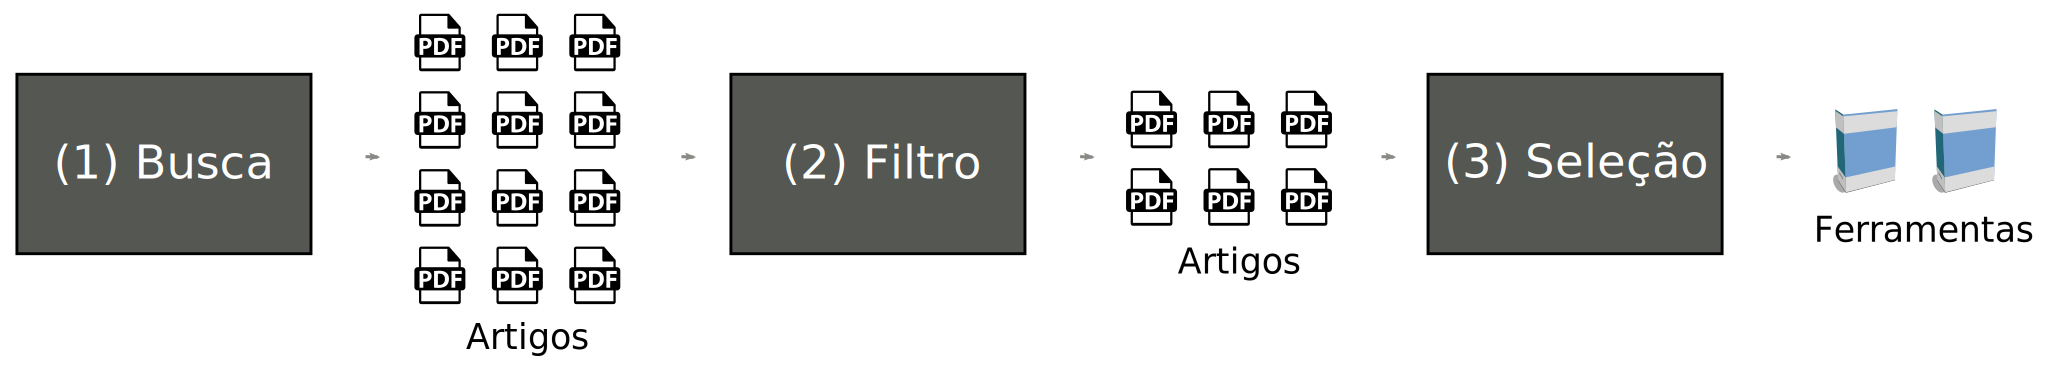
\includegraphics[scale=0.33]{imagens/revisao-estruturada.png}
  \caption{Representação gráfica da revisão estruturada}
  \label{figura-revisao-estruturada}
\end{figure}

A revisão estruturada é um processo disciplinado para seleção de artigos a
partir de critérios bem definidos, de forma que seja possível a reprodução do
estudo por parte de pesquisadores interessados.

A revisão está organizada em atividades de (1) busca de artigos (definição
das fontes de busca, definição de critérios de busca, definição de script de
busca, realização da busca nas fontes) e (2) seleção de artigos. 

No primeiro passo da revisão estruturada, as fontes de busca serão definidas,
considerando conferências que abordam o tema de interesse do estudo. 

A busca textual será realizada automaticamente, utilizando um
script\footnote{http://github.com/joenio/dissertacao-ufba-2016/blob/master/revisao-estruturada/filter}
escrito especialmente para este estudo. Esta busca seleciona os artigos que
contenham os seguintes termos:

\begin{verbatim}
  "tool" OU "framework"; E
  "download" OU "available"; E
  "http" OU "ftp"; E
  "static analysis" OU "parser".
\end{verbatim}

Uma cópia local de todos os artigos encontrados, em formato PDF, será feita.

No segundo passo, a seleção de artigos será feita com base nos artigos
encontrados pela busca no passo anterior.  Nesta seleção, pretende-se
identificar se cada artigo resulta, de fato, em publicação de ferramenta de
análise estática. Uma vez que se confirme que o artigo publica uma
ferramenta, este artigo será incluído para leitura. Ferramentas que sejam
mais abrangentes do que apenas análise estática mas que contenham esta função
em seu conjunto também serão selecionadas.

Uma vez identificados os artigos que publicaram ferramentas de análise
estática, procuramos no próprio artigo por referências de onde encontrar o
código-fonte da ferramenta. Neste contexto, algumas ações serão tomadas a
partir de algumas situações.

\begin{itemize}

  \item Se os autores afirmam que a ferramenta está disponível mas o artigo
    não contém referências de onde encontrar o código-fonte, então estes
    autores serão contactados, por email, solicitando informações de onde
    obter o código-fonte da ferramenta.

  \item Se o artigo indica onde obter o código-fonte da ferramenta, mas o acesso ao local
    indicado não está disponível, ou está disponível mas o software não se
    encontra lá, então os autores serão contactados, solicitando informações
    atualizadas de onde obter uma cópia do código-fonte da ferramenta.

  \item Artigos que indicam onde obter o código-fonte da ferramenta e a referência
    está correta. Será feito o download do código-fonte da última versão
    disponível.

\end{itemize}

Uma vez que os autores contactados por email respondam com informações sobre
local para obter o software, iremos adicionar a ferramenta ao conjunto de ferramentas
a serem analisadas.

Por fim, a ferramenta livre {\it
sloccount}\footnote{http://www.dwheeler.com/sloccount} será  utilizada para
identificar a linguagem de programação usada na implementação de cada
ferramenta selecionada.  A identificação da linguagem de programação é
necessária, pois apenas as ferramentas implementadas nas linguagens de
programação suportadas pela ferramenta Analizo serão consideradas.

\section{Coleta de dados} \label{coleta}

Serão realizadas duas etapas para identificar e mapear as ferramentas de
análise estática com código-fonte disponível: uma atividade para seleção de
ferramentas da academia, descrita na Seção \ref{ferramentas-da-academia}, e
outra atividade para seleção de ferramentas da indústria, descrita na Seção
\ref{ferramentas-da-industria}.

As ferramentas selecionadas para o estudo serão analisadas com Analizo para
extração dos valores de métricas de código-fonte.  Esta análise utilizará o
comando {\it metrics} do Analizo, que calcula métricas globais de projeto e
métricas por módulos. Este estudo levará em consideração a distribuição das
métricas por módulos.

\subsection{Ferramentas da academia} \label{ferramentas-da-academia}

A seleção de ferramentas da academia será relizada por meio de uma revisão
estruturada (seção~\ref{revisao-estruturada}). A fonte de busca para artigos
será a conferência SCAM - Source Code Analysis and Manipulation Working
Conference\footnote{http://www.ieee-scam.org} e mais uma dentre as seguintes
conferências:

\begin{itemize}
  \item ASE - Automated Software
    Engineering\footnote{http://ase-conferences.org}
  \item CSMR\footnote{A conferência CSMR tornou-se SANER - Software Analysis,
    Evolution, and Reengineering a partir da edição 2015.} - Conference on
    Software Maintenance and
    Reengineering\footnote{http://ansymore.uantwerpen.be/csmr-wcre}
  \item ICSME - International Conference on Software Maintenance and
    Evolution\footnote{http://www.icsme.org}
\end{itemize}

Todas estas conferências possuem trilhas para publicação de ferramentas e tem
como tema, áreas de estudo relacionadas à análise de programa e análise
estática, o que representa um grande potencial de encontrarmos ferramentas de
análise estática de código-fonte publicadas em suas mais de 20 edições. A
decisão de incluir apenas mais uma conferência além da conferência SCAM se
justifica pelo pouco tempo que temos para concluir este trabalho, de forma que
não seria viável incluir mais fontes.

Após download do código-fonte de cada ferramenta selecionada, em sua versão
mais recente, a ferramenta Analizo será utilizada para a coleta das métricas. 

\subsection{Ferramentas da indústria} \label{ferramentas-da-industria}

A seleção de ferramentas da indústria será feita de forma não estruturada a
partir de uma busca livre e manual no site do projeto SAMATE. As ferramentas
com código-fonte disponível, implementadas nas linguagens de programação
suportadas pelo Analizo serão selecionadas.

Após download do código-fonte de cada ferramenta selecionada, em sua versão
mais recente, a ferramenta Analizo será utilizada para a coleta das métricas. 

\section{Análise de dados} \label{analise}

Os dados coletados incluem métricas de código-fonte para cada módulo/classe de
cada ferramenta selecionada, tanto da indústria quanto da academia. As
métricas a serem analisadas e interpretadas são as métricas descritas na Seção
\ref{metricas-de-codigo}.

A linguagem R \cite{Ihaka1996}, uma linguagem de programação para cálculos
estatísticos e gráficos, será utilizada para manipulação de dados, criação de
tabelas e plotagem de gráficos. Todos os cálculos em linguagem R utilizados
neste trabalho estão disponíveis
em nosso repositório\footnote{https://github.com/joenio/dissertacao-ufba-2016/blob/master/qualificacao.R}.

\subsection{Distribuição dos valores das métricas}

Iremos calcular os percentis de cada métrica para cada ferramenta a partir dos
valores das métricas dos seus módulos, um percentil é a centésima parte dos
dados ordenados de forma crescente, iremos calcular os percentis 1, 5, 10, 25,
50, 75, 90, 95 e 99, e dentre eles iremos discutir os resultados em função dos
percentis 75, 90 e 95, assim como feito por \citeonline{Meirelles2013},
correspondendo a valores muito frequentes, frequentes e pouco frequentes,
respectivamente.

Esta discussão irá nos fornecer como resultado intervalos de referência para
métricas de código-fonte neste domínio de aplicação, estes intervalos serão
definidos a partir da interpretação manual dos percentis e serão analisados
usando modelos de regressão a fim de serem compreendidos e validados, uma
comparação com intervalos encontrados nos trabalhos relacionados (seção
\ref{trabalhos-relacionados}) também será realizada com objetivo de reforçar
estes valores.

\subsection{Cálculo de distância e modelo de aproximação} \label{distancia}

A partir da distribuição das métricas nos percentis 75, 90 e 95 e dos
intervalos de referência encontrados propomos uma abordagem para calcular o
quão distante cada ferramenta se encontra destes intervalos.  Esta abordagem
terá como base um fator de aproximação chamado {\it score} de similaridade,
este {\it score} será primeiramente calculado para os intervalos de referência
e servirão como base de comparação para o cálculo da distância de cada
ferramenta.

O {\it score} de similaridade será calculado a nível de projeto, ou seja,
teremos um único valor para cada ferramenta calculado a partir de suas várias
métricas. Para isto, iremos abstrair o significado individual de cada métrica,
o que pode não ser muito efetivo já que diferentes métricas possuem diferentes
grandezas. Para resolver este problema será feita uma normalização dos valores
das várias métricas a fim de deixá-las num mesmo intervalo, com uma certa
equivalência, seguindo uma ideia semelhante ao que é feito com a distância
euclidiana, onde todas as variáveis tem suas distâncias unificadas em um único
valor.

Os valores do {\it score} calculados a partir dos intervalos de referência
serão centralizados em 0, indicando o centro de comparação para o cálculo da
distância com cada ferramenta, desta forma, ferramentas com {\it score} acima
de 0 indicam valores piores em relação aos intervalos de referência, e
ferramentas com {\it score} abaixo de 0 indicam valores melhores do que os
intervalos de referência.

\subsection{Caracterização das ferramentas} \label{caracterizacao-das-ferramentas}

\citeonline{Novak2010} através de um estudo para construção de uma taxonomia
para ferramentas de análise estática propuseram uma classificação a partir de
uma série de categorias.

\begin{description}

  \item {\it Entrada - quais tipos de arquivos podem ser carregados na ferramenta:}
    \begin{itemize}
      \item Código-fonte - arquivos de código texto podem ser carregados
      \item Byte code - arquivos com Java Byte Code ou Microsoft
      \item Linguagem intermediária (MSIL) pode ser carregada
    \end{itemize}

  \item {\it Lançamentos ({\it Releases}) - quantos lançamentos por ano:}
    \begin{itemize}
      \item Frequentemente $>=$ 3 vezes ao ano - novas versões da ferramenta são lançadas 3 ou mais vezes por ano
      \item Ocasionalmente $<$ 3 vezes ao ano - novas versões da ferramenta são lançadas menos que 3 vezes ao ano
      \item Obsoleta 0 vezes ao ano - intervalo entre novos lançamentos é maior que 1 ano
    \end{itemize}

  \item {\it Linguagens suportadas - quais linguagens de programação a ferramenta suporta:}
    \begin{itemize}
      \item .NET - todas as linguagens compiladas em bibliotecas ou programas no framework .NET
      \item VB .NET - suporta VB.NET
      \item C\# - suporta C\#
      \item Java - suporta linguagem de programação Java
      \item C, C++ - suporta linguagem de programação C ou C++
    \end{itemize}

  \item {\it Tecnologia - quais tecnologias são usadas para procurar erros no código:}
    \begin{itemize}
      \item Dataflow - busca por erros com dataflow
      \item Sintaxe - busca por errors de sintaxe e correctness
      \item Prova de teoremas - procurar erros em provar diferentes teoremas
      \item Verificação de modelos - procurar erros com verificação de modelo
    \end{itemize}

  \item {\it Regras - conjunto de regras, quais são suportadas por diferentes código estático:}
    \begin{itemize}
      \item Estilo - inspeciona a aparência do código-fonte
      \item Naming - checa se as varáveis são nomeadas corretamente (ortografia, padroes de nomenclatura, ...)
      \item Geral - regras gerais de analise estática de código
      \item Concorrencia - erros com execução de código de concorrente
      \item Exceções - erros lançando ou não exceções
      \item Performance - erros de performance das aplicações
      \item Interoperabilidade - erros de comportamento comum
      \item Segurança - erros que podem impactar na segurança da aplicação
      \item SQL - procurar por "SQL injections" e outros erros de SQL
      \item Buffer overflow - erros de segurança, que explorar buffer overflow
      \item Manutenabilidade - regras para melhor manutenabilidade da aplicação
    \end{itemize}

  \item {\it Configurabilidade - habilidade de configurar a ferramenta:}
    \begin{itemize}
      \item Documento texto - comfiguração é feita via documento texto
      \item XML - configuração pe feita por documento XML
      \item GUI - configuraçãi é feita via interface gráfica
      \item Ruleset - ferramenta pode ligar/desligar conjunto de regras
    \end{itemize}

  \item {\it Extensibilidade - se a ferramenta pode ser extendida com regras próprias:}
    \begin{itemize}
      \item Possível - é possível extender
      \item Não possível - não é possível extender
    \end{itemize}

  \item {\it Disponibilidade - de que forma a ferramenta está disponível:}
    \begin{itemize}
      \item Código Aberto ({\it Open Source}) - a ferrament é livre e o código-fonte está disponível
      \item Grátis ({\it Free}) - a ferramenta é grátis mas o código-fonte não está disponível
      \item Comercial - a ferramenta está disponível mediante pagamento
    \end{itemize}

  \item {\it Experiência do usuário - de que forma a ferramenta pode ser usada, como é oferecida:}
    \begin{itemize}
      \item Integração com ambiente - como a ferramenta é integrada ao ambiente de trabalho
      \item Localização automática de erros no código - quando a ferramenta encontra um erro, ela leva ao local do erro
      \item Ajuda abrangente sobre falhas - se a ferramenta oferece ajuda na resolução de erros
      \item Interface de usuário - disponibilidade de uma interface de usuário
      \item Linha de comando - ela pode ser executada via linha de comando
      \item GUI - a ferramente pode ser executada em uma interface gráfica (GUI)
    \end{itemize}

  \item {\it Saída - representação dos resultados da ferramenta:}
    \begin{itemize}
      \item Arquivo texto - ferramenta pode apresentar resultados em arquivos texto
      \item Lista - ferramenta pode apresentar resultados numa interface de usuário customizada controlada em GUI
      \item Arquivo XML - ferramenta pode apresentar resultados em dados XML
      \item Arquivo HTML - ferramenta pode apresentar resultados em dados HTML
    \end{itemize}

\end{description}

Iremos utilizar algumas destas categorias na caracterização das ferramentas
selecionadas neste estudo, e vamos também caracterizar em relação à linguagem de
programação a qual foi escrita.

O Apêndice \ref{caracterizacao-ferramentas} traz uma caracterização inicial
das ferramentas segundo às categorias acima.

\section{Cronograma} \label{cronograma}

\begin{table}[h!]
  \centering
  \begin{tabular}{| l | c | c | c | c | c |}
    \hline
    {\bf Atividade}                                & Jul     & Ago       & Set      & Out      & Nov      \\
    \hline
    \hline
    Qualificação                                   &\checkmark&          &          &          &          \\
    \hline
    Análise da distribuição das métricas           &\checkmark&          &          &          &          \\
    \hline
    Definição dos valores de referência            &          &\checkmark&          &          &          \\
    \hline
    Cálculo de distância e modelo de aproximação   &          &\checkmark&          &          &          \\
    \hline
    Revisão estruturada com mais uma conferência   &          &\checkmark&          &          &          \\
    \hline
    Adicionar coleta/análise com novas ferramentas &          &          &\checkmark&          &          \\
    \hline                                                                                     
    Caracterização das ferramentas                 &          &          &\checkmark&          &          \\
    \hline                                                                                     
    Caracterização da complexidade estrutural      &          &          &          &\checkmark&          \\
    \hline                                                                                     
    Evolução da ferramenta Analizo                 &\checkmark&\checkmark&\checkmark&\checkmark&\checkmark\\
    \hline
    Defesa                                         &          &          &          &          &\checkmark\\
    \hline
  \end{tabular}
\end{table}
